\documentclass[smaller,handout]{beamer}
%\documentclass[smaller]{beamer}

\usepackage{amsfonts}
\usepackage{amssymb}
\usepackage{amsmath}
\usepackage{epsfig}
\usepackage{graphicx}
\usepackage{empheq}

\def\F{{\cal F}}
\def\X{{\cal X}}
\def\Y{{\cal Y}}
\def\Z{{\cal Z}}
\def\P{{\mathbb P}}
\def\R{{\mathbb R}}
\def\E{{\mathbb E}}
\def\bZ{{\mathbb Z}}
\def\darkred{\color{red!70!black}}
\def\darkgreen{\color{green!60!black}}
\def\learn{{\mbox{LEARN}}}
\def\err{{\mbox{err}}}
\def\bI{{\tilde{I}}}
\def\dis{{\mbox{DIS}}}

\DeclareMathOperator*{\argmin}{arg\,min}
\DeclareMathOperator*{\argmax}{arg\,max}

\usepackage{pgfpages}
\pgfpagesuselayout{4 on 1}[letterpaper,border shrink=5mm,landscape]

%\usepackage{beamerarticle}

\mode<presentation>
{
  \usetheme{default}
%  \setbeamercovered{transparent}
  % or whatever (possibly just delete it)
}


\usepackage[english]{babel}
% or whatever

\useinnertheme{circles}
\usefonttheme{structurebold}

%\usepackage[latin1]{inputenc}
% or whatever

%\usepackage{times}
%\usepackage[T1]{fontenc}
% Or whatever. Note that the encoding and the font should match. If T1
% does not look nice, try deleting the line with the fontenc.

\title{More linear classification}

\author{CSE 250B}
% - Give the names in the same order as the appear in the paper.
% - Use the \inst{?} command only if the authors have different
%   affiliation.

%\institute{University of California, San Diego}

\date{}

% If you wish to uncover everything in a step-wise fashion, uncomment
% the following command: 

%\beamerdefaultoverlayspecification{<+->}
\setbeamertemplate{navigation symbols}{}

\def\vone{{\vskip.1in}}
\def\v2{{\vskip.2in}}
\def\bR{{\mathbb R}}
\def\R{{\mathbb R}}
\def\eps{{\epsilon}}
\def\E{{\mathbb E}}
\def\epso{{\epsilon_o}}
\def\nicered{{\color{red!70!black}}}
\def\pr{{\mbox{\rm Pr}}}

\setbeamercolor{title}{fg=red!80!black,bg=red!20!white}
\setbeamercolor{author}{fg=blue!80!black}

\begin{document}

% *** TITLE ***
\begin{frame}
  \titlepage
\end{frame}

% *** THE DECISION BOUNDARY ***
\begin{frame}
\frametitle{The decision boundary}

\begin{center}
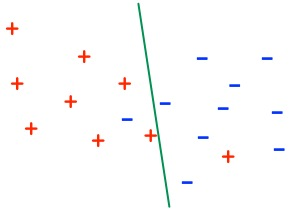
\includegraphics[width=2in]{discriminative.jpg}
\end{center}

\v2
{\darkred Decision boundary in $\R^p$ is a {\bf hyperplane}.}
\begin{itemize}
\item How is this boundary parametrized?
\item How can we learn a hyperplane from training data?
\end{itemize}

\end{frame}

% *** HYPERPLANES ***
\begin{frame}
\frametitle{Hyperplanes}


\raisebox{1in}{
\begin{minipage}[t]{2in}
Hyperplane $\{x: w \cdot x = b\}$
\begin{itemize}
\item orientation $w \in \R^p$ 
\item offset $b \in \R$ 
\end{itemize}
\end{minipage}}
\hskip.2in
\includegraphics[width=1.75in]{hyperplane.pdf}

\pause\v2
{\darkgreen Can always normalize $w$ to unit length:
\begin{align*}
(w,b) \ \ \ 
&\longleftrightarrow 
\ \ \ \left(\widehat{w} = \frac{w}{\|w\|}, \frac{b}{\|w\|} \right) \\
w \cdot x = b \ \ \ 
&\longleftrightarrow
\ \ \ \widehat{w} \cdot x = \frac{b}{\|w\|}
\end{align*}}

\pause
\alert{Equivalently: all points whose projection onto $\widehat{w}$ is $b/\|w\|$.}

\end{frame}

% *** HOMOGENEOUS LINEAR SEPARATORS ***
\begin{frame}
\frametitle{Homogeneous linear separators}

{\darkred Hyperplanes that pass through the origin have no offset, $b=0$.}

\pause\vone
Reduce to this case by adding an extra feature to $x$:
$$ \widetilde{x} = (x,1) \in \R^{p+1} $$
Then $\{x: w \cdot x = b\} \equiv \{x: \widetilde{w} \cdot \widetilde{x} = 0\}$ where $\widetilde{w} = (w,-b)$.

\pause
\begin{center}
\includegraphics[width=3.25in]{homogeneous1.pdf}
\end{center}

\end{frame}

% *** THE LEARNING PROBLEM: SEPARABLE CASE ***
\begin{frame}
\frametitle{The learning problem: separable case}

{\darkred
{\it Input:} training data $(x^{(1)}, y^{(1)}), \ldots, (x^{(n)}, y^{(n)}) \in \R^p \times \{-1,+1\}$

\vone
{\it Output:} linear classifier $w \in \R^p$ such that
$$ y^{(i)} (w \cdot x^{(i)}) > 0 \mbox{\ \ \ for $i = 1, 2, \ldots, n$} $$}

\pause
{\darkgreen This is linear programming:}
\begin{itemize}
\item {\darkgreen Each data point is a linear constraint on $w$}
\item {\darkgreen Want to find $w$ that satisfies all these constraints}
\end{itemize}
{\darkgreen But we won't use generic linear programming methods, such as simplex.}

\pause\v2
A simple alternative: {\bf Perceptron algorithm} (Rosenblatt, 1958)
\begin{itemize}
\item $w = 0$
\item while some $(x,y)$ is misclassified:
\begin{itemize}
\item $w = w + yx$
\end{itemize}
\end{itemize}

\end{frame}

% *** PERCEPTRON: EXAMPLE ***
\begin{frame}
\frametitle{Perceptron: example}

\begin{itemize}
\item $w = 0$
\item while some $(x,y)$ is misclassified:
\begin{itemize}
\item $w = w + yx$
\end{itemize}
\end{itemize}

\begin{center}
\raisebox{1in}{\includegraphics[width=.5in]{legend.pdf}}
\hskip.25in
%\includegraphics<1>[width=2.5in]{perc1.pdf}
%\includegraphics<2>[width=2.5in]{perc2.pdf}
\includegraphics<3>[width=2.5in]{perc3.pdf}
\end{center}

\alert{{\bf Separator: \only<1>{$w = 0$}\only<2>{$w=-x^{(1)}$}\only<3>{$w = -x^{(1)} + x^{(6)}$}}}

\end{frame}

% *** PERCEPTRON: CONVERGENCE ***
\begin{frame}
\frametitle{Perceptron: convergence}

{\darkred
{\bf Theorem:} Let $R = \max \|x^{(i)}\|$. Suppose there is a unit vector $w^*$
and some (margin) $\gamma > 0$ such that
$$ y^{(i)} (w^* \cdot x^{(i)}) \geq \gamma \mbox{\ \ for all $i$}.$$
Then the Perceptron algorithm converges after at most $R^2/\gamma^2$ updates.}

\v2\pause
{\darkgreen \bf Proof idea.} {\darkgreen Let $w_t$ be the classifier after $t$ updates.}

\v2

\hskip.5in
\includegraphics[width=1in]{perceptronproof.pdf}
\hskip.25in
\raisebox{.2in}{\begin{minipage}[b]{2in}
{\darkgreen {\bf Track angle between $w_t$ and $w^*$}:
$$ \cos(\angle(w_t,w^*)) = \frac{w_t \cdot w^*}{\|w\|} .$$}
\end{minipage}}

\pause\v2
On each mistake, when $w_t$ is updated to $w_{t+1}$,
\begin{itemize}
\item $w_t \cdot w^*$ grows significantly.
\item $\|w_t\|$ does not grow much.
\end{itemize}

\end{frame}

% *** PERCEPTRON CONVERGENCE, CONT'D ***
\begin{frame}
\frametitle{Perceptron convergence, cont'd}

{\darkred Perceptron update: if $y(w_t \cdot x) < 0$ (misclassified) then $w_{t+1} = w_t + yx$.

Target vector $w^*$ has unit length, and margin condition $y(w^* \cdot x) \geq \gamma$.}

\begin{enumerate}
\item<2-> Initial vector $w_0 = 0$.
\item<3-> When updating $w_t$ to $w_{t+1}$:
\begin{align*}
w_{t+1} \cdot w^* &= (w_t + yx) \cdot w^* = w_t \cdot w^* + y (w^* \cdot x) \geq w_t \cdot w^* + \gamma \\
\onslide<4->{\|w_{t+1}\|^2 &= \|w_t + yx\|^2 = \|w_t\|^2 + \|x\|^2 + 2 y(w_t \cdot x) \leq \|w_t\|^2 + R^2}
\end{align*}
\item<5-> After $T$ updates, we have 
\begin{align*}
w_T \cdot w^* &\geq T \gamma \\
\|w_T\|^2 &\leq TR^2
\end{align*}
\item<6-> The angle between $w_T$ and $w^*$ is given by
$$\cos(\angle(w_T,w^*)) = \frac{w_T \cdot w^*}{\|w\|} \geq \frac{T\gamma}{R\sqrt{T}} .$$
{\darkgreen\bf This is at most $1$, so $T \leq R^2/\gamma^2$.}
\end{enumerate}
\end{frame}

% *** A BETTER SEPARATOR? ***
\begin{frame}
\frametitle{A better separator?}

For a linearly separable data set, there are in general many possible separating hyperplanes, and
Perceptron is guaranteed to find one of them. 

\v2
\begin{center}
\includegraphics[width=1.75in]{choices.pdf}
\end{center}

\pause\v2
\alert{But is there a better, more systematic choice of separator? The one with the most buffer around it, for instance?}

\end{frame}

% *** MAXIMIZING THE MARGIN ***
\begin{frame}
\frametitle{Maximizing the margin}

Given training data $(x^{(1)}, y^{(1)}), \ldots, (x^{(n)}, y^{(n)}) \in \R^p \times \{-1,+1\}$, find $w \in \R^p$ and $b \in \R$ such that
$y^{(i)}(w \cdot x^{(i)} + b) > 0$ for all $i$.

\pause\vone
{\darkred By scaling $w,b$, can equally ask for 
$$ y^{(i)}(w \cdot x^{(i)} + b) \geq 1 \mbox{\ \ \ for all $i$} .$$}

\pause\vone
\begin{center}
\includegraphics[width=3in]{margin.pdf}
\end{center}

\pause\alert{Maximize the {\bf margin} $\gamma$.}
\end{frame}

% *** WHAT IS THE MARGIN? ***
\begin{frame}
\frametitle{What is the margin?}

{\darkred Close-up of a point $z$ on the positive boundary.}

\begin{center}
\includegraphics[width=2.5in]{margin2.pdf}
\end{center}

\pause
Let $\widehat{w}$ be the unit vector in the direction of $w$, i.e. $\widehat{w} = w/\|w\|$.

\pause
Then $z - \gamma \widehat{w}$ is on the separator, so
$$ w \cdot (z - \gamma \widehat{w}) + b = 0
\ \ \Rightarrow \ \ 
\gamma w \cdot \widehat{w} = w \cdot z + b = 1
\ \ \Rightarrow \ \ 
\gamma = 1/\|w\|$$

\pause\vone
\alert{In short: to maximize the margin, minimize $\|w\|$.}

\end{frame}

% *** MAXIMUM-MARGIN LINEAR CLASSIFIER ***
\begin{frame}
\frametitle{Maximum-margin linear classifier}

\begin{itemize}
\item<1-> Given $(x^{(1)}, y^{(1)}), \ldots, (x^{(n)}, y^{(n)}) \in \R^p \times \{-1,+1\}$.

{\darkred
\begin{empheq}[box=\fbox]{gather}
(\text{\sc primal})\ \ \ \  \min_{w \in \R^p, b \in \R} \ \ \frac{1}{2} \|w\|^2 \hskip1in \nonumber \\
\mbox{s.t.:\ \ } y^{(i)}(w \cdot x^{(i)} + b) \geq 1 \mbox{\ \ \ for all $i=1,2,\ldots,n$} \nonumber
\end{empheq}}

\item<2-> This is a convex optimization problem:
\begin{itemize}
\item Convex objective function
\item Linear constraints
\end{itemize}
\item<3-> It has a dual maximization problem with the same optimum value.

{\darkred
\begin{empheq}[box=\fbox]{gather}
(\text{\sc dual}) \ \ \ \ \max_{\alpha \in \R^n} \ \ \sum_{i=1}^n \alpha_i - \frac{1}{2} \sum_{i,j=1}^n \alpha_i \alpha_j y^{(i)} y^{(j)} (x^{(i)} \cdot x^{(j)})  \nonumber \\
\mbox{s.t.:\ \ } \sum_{i=1}^n \alpha_i y^{(i)} = 0 \nonumber \\
\alpha \geq 0 \nonumber
\end{empheq}}
\end{itemize}

\end{frame}

% *** COMPLEMENTARY SLACKNESS ***
\begin{frame}
\frametitle{Complementary slackness}

{\darkred
\begin{empheq}[box=\fbox]{gather}
(\text{\sc primal})\ \ \ \  \min_{w \in \R^p, b \in \R} \ \ \frac{1}{2} \|w\|^2 \hskip1in \nonumber \\
\mbox{s.t.:\ \ } y^{(i)}(w \cdot x^{(i)} + b) \geq 1 \mbox{\ \ \ for all $i=1,2,\ldots,n$} \nonumber
\end{empheq}}

{\darkred
\begin{empheq}[box=\fbox]{gather}
(\text{\sc dual}) \ \ \ \ \max_{\alpha \in \R^n} \ \ \sum_{i=1}^n \alpha_i - \frac{1}{2} \sum_{i,j=1}^n \alpha_i \alpha_j y^{(i)} y^{(j)} (x^{(i)} \cdot x^{(j)})  \nonumber \\
\mbox{s.t.:\ \ } \sum_{i=1}^n \alpha_i y^{(i)} = 0 \nonumber \\
\alpha \geq 0 \nonumber
\end{empheq}}

At optimality, $w = \sum_{i=1}^n \alpha_i y^{(i)} x^{(i)}$ and moreover
$$
\alpha_i > 0  \ \ \Rightarrow \ \ y^{(i)}(w \cdot x^{(i)} + b) = 1
$$
Points $x^{(i)}$ with $\alpha_i > 0$ are called {\bf support vectors}.

\end{frame}

% *** SUPPORT VECTORS ***
\begin{frame}
\frametitle{Support vectors}

\begin{center}
\includegraphics[width=3in]{margin3.pdf}
\end{center}

\v2
Linear classifier $w = \sum_{i=1}^n \alpha_i y^{(i)} x^{(i)}$ is a function of just the support vectors.

\end{frame}

% *** SMALL EXAMPLE: IRIS ***
\begin{frame}
\frametitle{Small example: Iris data set}

\begin{center}
%\includegraphics<1>[width=3in]{iris0.png}
\includegraphics<2>[width=3in]{iris10.png}
\end{center}

\end{frame}


% *** THE NON-SEPARABLE CASE ***
\begin{frame}
\frametitle{The non-separable case}

Idea: allow each data point $x^{(i)}$ some slack $\xi_i$.

{\darkred
\begin{empheq}[box=\fbox]{gather}
(\text{\sc primal})\ \ \ \  \min_{w \in \R^p, b \in \R, \xi \in \R^n} \ \ \frac{1}{2} \|w\|^2 + C \sum_{i=1}^n \xi_i  \nonumber \\
\mbox{s.t.:\ \ } y^{(i)}(w \cdot x^{(i)} + b) \geq 1-\xi_i \mbox{\ \ \ for all $i=1,2,\ldots,n$} \nonumber \\
\xi \geq 0 \nonumber
\end{empheq}}

\begin{center}
\includegraphics[width=2.5in]{slack.pdf}
\end{center}

\end{frame}

% *** DUAL FOR GENERAL CASE ***
\begin{frame}
\frametitle{Dual for general case}

{\darkred
\begin{empheq}[box=\fbox]{gather}
(\text{\sc primal})\ \ \ \  \min_{w \in \R^p, b \in \R, \xi \in \R^n} \ \ \frac{1}{2} \|w\|^2 + C \sum_{i=1}^n \xi_i  \nonumber \\
\mbox{s.t.:\ \ } y^{(i)}(w \cdot x^{(i)} + b) \geq 1-\xi_i \mbox{\ \ \ for all $i=1,2,\ldots,n$} \nonumber \\
\xi \geq 0 \nonumber
\end{empheq}}

{\darkred
\begin{empheq}[box=\fbox]{gather}
(\text{\sc dual}) \ \ \ \ \max_{\alpha \in \R^n} \ \ \sum_{i=1}^n \alpha_i - \frac{1}{2}\sum_{i,j=1}^n \alpha_i \alpha_j y^{(i)} y^{(j)} (x^{(i)} \cdot x^{(j)})  \nonumber \\
\mbox{s.t.:\ \ } \sum_{i=1}^n \alpha_i y^{(i)} = 0 \nonumber \\
0 \leq \alpha_i \leq C \nonumber
\end{empheq}}

At optimality, $w = \sum_i \alpha_i y^{(i)} x^{(i)}$, with
\begin{align*}
0 < \alpha_i < C \ \ &\Rightarrow \ \ y^{(i)}(w \cdot x^{(i)} + b) = 1 \\
\alpha_i = C     \ \ &\Rightarrow \ \ y^{(i)}(w \cdot x^{(i)} + b) = 1 - \xi_i 
\end{align*}
\end{frame}

% *** WINE DATA SET ***
\begin{frame}
\frametitle{Wine data set}

{\darkred Here $C = 1.0$}

\v2

\begin{center}
%\includegraphics<1>[width=3in]{wine0.png}
\includegraphics<2>[width=3in]{winesvm1.png}
\end{center}

\end{frame}

% *** BACK TO IRIS ***
\begin{frame}
\frametitle{Back to Iris}

{\darkred 
%\only<1-2>{$C = 10$}
%\only<3>{$C = 3$}
%\only<4>{$C = 2$}
%\only<5>{$C = 1$}
%\only<6>{$C = 0.5$}
%\only<7>{$C = 0.1$}
\only<8>{$C = 0.01$}
}

\v2
\begin{center}
%\includegraphics<1>[width=3in]{iris0.png}
%\includegraphics<2>[width=3in]{iris10.png}
%\includegraphics<3>[width=3in]{iris3.png}
%\includegraphics<4>[width=3in]{iris2.png}
%\includegraphics<5>[width=3in]{iris1.png}
%\includegraphics<6>[width=3in]{iris05.png}
%\includegraphics<7>[width=3in]{iris01.png}
\includegraphics<8>[width=3in]{iris001.png}
\end{center}

\end{frame}

% *** CONVEX SURROGATES FOR 0-1 LOSS ***
\begin{frame}
\frametitle{Convex surrogates for 0-1 loss}

{\darkred Want a separator $w$ that misclassifies as few training points as possible. }
\begin{itemize}
\item {\darkred 0-1 loss: charge $1(y (w \cdot x) < 0)$ for each $(x,y)$}
\end{itemize}
{\darkred Problem: this is NP-hard.}

\pause\vone
Instead, use {\bf convex} loss functions.
\begin{itemize}
\item Hinge loss (SVM): charge $(1- y(w \cdot x))_+$
\item Logistic loss: charge $\ln (1 + e^{-y(w \cdot x)})$ 
\end{itemize}

\pause
\begin{center}
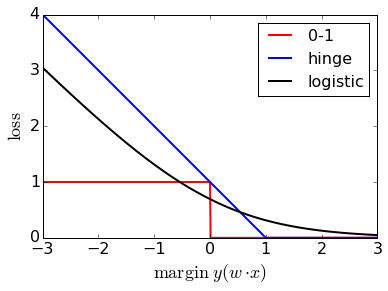
\includegraphics[width=2.5in]{loss-functions.png}
\end{center}

\end{frame}

% *** A HIGH-LEVEL VIEW OF OPTIMIZATION ***
\begin{frame}
\frametitle{A high-level view of optimization}

\alert{\bf Unconstrained optimization}

Logistic regression: find the vector $w \in \R^p$ that minimizes
$$ L(w) = \sum_{i=1}^n \ln (1 + \exp(- y^{(i)} (w \cdot x^{(i)})) .$$
{\darkgreen We know how to check such problems for convexity and how to solve using gradient descent or Newton methods.}

\pause\v2
\alert{\bf Constrained optimization}

Support vector machine: find $w \in \R^p$ and $b \in \R$ that minimize
$$ L(w) = \|w\|^2$$
subject to the constraints
$$ y^{(i)} (w \cdot x^{(i)} + b) \geq 1 $$
{\darkgreen What problems of this kind are easy to solve?}

\end{frame}

% *** CONSTRAINED OPTIMIZATION ***
\begin{frame}
\frametitle{Constrained optimization}

{\darkred Write the optimization problem in a standardized form:
\begin{gather*}
\min f_o(z) \\
f_i(z) \leq 0 \mbox{\ \ for $i=1,..,m$} \\
h_i(z) = 0    \mbox{\ \ for $i=1,..,n$}
\end{gather*}}

Special cases that can be solved (relatively) easily:
\begin{itemize}
\item {\bf Linear programs.}

{\darkgreen $f_o, f_i, h_i$ are all linear functions.}

\item {\bf Convex programs.}

{\darkgreen $f_o, f_i$ are convex functions. The $h_i$ are linear functions.}

\end{itemize}

\end{frame}

% *** EXAMPLE: REGRESSION WITH ELL_1 LOSS ***
\begin{frame}
\frametitle{Example: regression with $\ell_1$ loss}

{\darkred Given $(x^{(1)}, y^{(1)}), \ldots, (x^{(n)}, y^{(n)}) \in \R^p \times \R$, find $w \in \R^p$ minimizing
$$ L(w) = \sum_{i=1}^n |y^{(i)} - (w \cdot x^{(i)})| .$$}

\pause\vskip.05in
{\darkgreen Equivalently: let $X$ be the $n \times p$ matrix with rows $x^{(i)}$, and $y = (y^{(1)}, \ldots, y^{(n)})$. Then
$ L(w) = \|Xw - y\|_1 .$}

\pause\v2
Optimization problem in $p+n$ variables, $w \in \R^p$ and $z \in \R^n$:
\begin{gather*}
\min \sum_{i=1}^n z_i \\
y^{(i)} - w \cdot x^{(i)} \leq z_i, \ \ \ i = 1, 2, \ldots, n \\
w \cdot x^{(i)} - y^{(i)} \leq z_i, \ \ \ i = 1, 2, \ldots, n
\end{gather*}

\pause
\alert{A linear program.}

\end{frame}

% *** THE DUAL OF AN OPTIMIZATION PROBLEM ***
\begin{frame}
\frametitle{The dual of an optimization problem}

Take any optimization problem, convex or not:
\begin{gather*}
\min f_o(z) \\
f_i(z) \leq 0 \mbox{\ \ for $i=1,..,m$} \\
h_i(z) = 0    \mbox{\ \ for $i=1,..,n$}
\end{gather*}
Call this the {\it primal} problem.

\pause\v2
{\darkred 
There is a {\it dual} optimization problem over $n+m$ variables:
\begin{itemize}
\item {\darkred $\lambda \in \R^m$, one variable for each primal inequality}
\item {\darkred $\nu \in \R^n$, one variable for each primal equality}
\end{itemize}
It is a maximization problem:
\begin{gather*}
\max \, g(\lambda, \nu) \\
\lambda \geq 0
\end{gather*}}

\pause
{\darkgreen Constructing the dual is straightforward. But interpreting it is not.}

\end{frame}

% *** DUALITY AND COMPLEMENTARY SLACKNESS ***
\begin{frame}
\frametitle{Duality and complementary slackness}

{\darkgreen Let $z^*$ and $\lambda^*, \nu^*$ be the optimal primal and dual solutions.}

\begin{itemize}
\item<2-> {\darkred Weak duality.}

Dual solution is at most the primal solution: $g(\lambda^*, \nu^*) \leq f_o(z^*)$.

\item<3-> {\darkred Strong duality.}

If primal problem is convex then (almost always, with an easily checkable condition) the primal and dual solutions are equal.

\item<4-> {\darkred Complementary slackness.}

If primal and dual solutions are equal, then for any $i = 1, \ldots, m$,
$$ \lambda_i^* > 0 \ \Rightarrow \ f_i(z^*) = 0 .$$

\item<5-> {\darkred KKT (Karush-Kuhn-Tucker) conditions.}

If the $f_i$ and $h_i$ are differentiable, these are first-derivative-equals-zero conditions that hold at optimality.


\end{itemize}

\end{frame}


\end{document}
